\label{sec:detectfalseshare}

This section first describes the basic idea of detecting false sharing. 

\subsection{Basic Idea}
\label{sec:detectionidea}

There is a false sharing problem when two threads concurrently access independent data within the same cache line. False sharing does not necessarily cause performance problems. It can greatly degrade performance only when those accesses, caused by threads running on different cores with separate cache, actually cause a big number of cache invalidations. This is our \textbf{basic observation}. 

But it is not a easy task to know how many cache invalidations actually happen on a specific cache line. Generally, there are two ways to know this type of information. The first approach should rely on the underlying hardware. For example, we may rely on specific hardware performance counters, existing in some special hardware but not all, to know how many cache invalidations happening on a specific cache line. However, relying on the hardware-based approach to track cache invalidations can greatly reduce a tool's portability, which can not simply apply the same tool to different hardware. Also, those hardware-based mechanisms may not present complete invalidation information on all cache lines. Most of existing hardwares only sample those information for a performance purpose. 

The second approach is to utilize simulation to simulate the activity on different cache lines, thus provide some simulation results on cache invalidations. Developing simulation has to know all hardware-related information, including cache hierarchy, cache capacity and cache eviction rule, and the relationship between a thread and a specific core.  However, simulation-based approaches are normally very slow and cannot be generalized to different hardware environment. 

We avoid these approaches because of their unavoidable shortcomings. For example, it is hard to know where a thread is located in the user space. Moreover, it is unnecessary to know this relationship since the relationship between threads and cores can be changed from one execution to the other. Thus, we make the \textbf{ first assumption}: all threads are running on different cores, with separate caches. Thus we can report the potential worst-case results that can caused by false sharing problems inside. Also, using this assumption can avoid knowing actual hardware cache hierarchy. 

But this simple assumption is not enough to know how many cache invalidations happening on a cache line. For example, cache invalidations on a cache line are also affected by a cache's capacity and specific eviction rule. Thus, we further assume (\textbf{second assumption}) that the data is never evicted from its private cache by cache eviction. This means that all caches have infinite capacity. 

These two assumptions allow us to get cache invalidations based on memory accesses only, no need to think about hardware information. Based on these assumptions, there is a cache invalidation if a processor writes a cache line after another thread's access on the same cache line. Because the last thread accessing this cache line creates a copy of the same cache line on its running core's private cache (first assumption) and  holds this copy(second assumption), this write operation definitely cause a cache invalidation before or after this write operation, depending on different cache coherence protocols. 


\begin{figure}[!t]
\centering
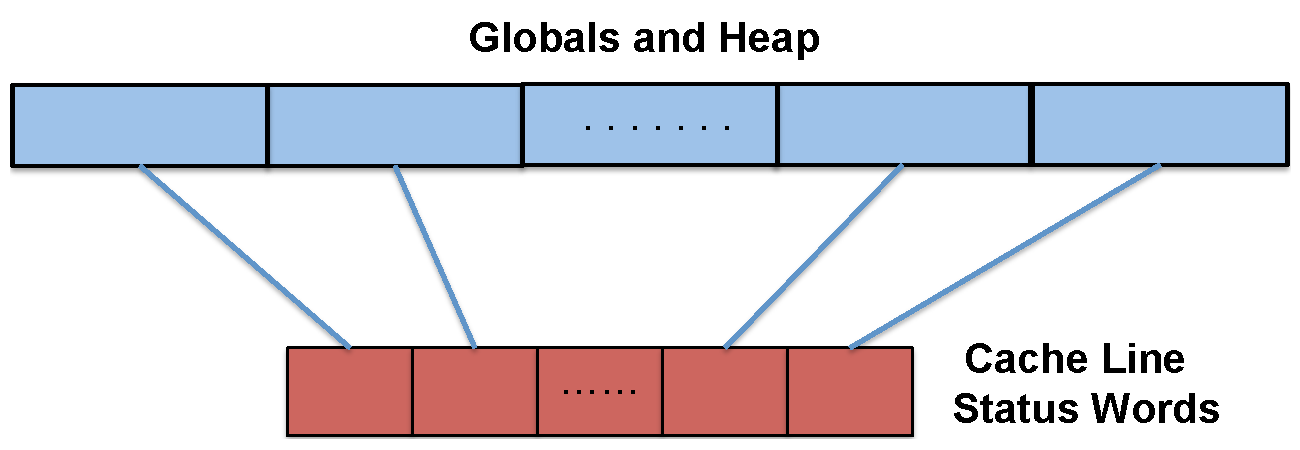
\includegraphics[width=6in]{fig/cachelinestatuswords}
\caption{
To detect false sharing, each cache line of the globals and heap maintains a cache line status word, which is updated on each tracked memory access. \label{fig:cachelinestatusword}}
\end{figure}


To locate cache lines with a big number of cache invalidations, we maintain a cache line status word for each cache line in the globals and heap, shown in Figure~\ref{fig:cachelinestatusword}. We share a similar mechanism as another concurrent work of Zhao et.al. ~\cite{qinzhao}. 
However, the detailed implementation is totally different. Zhao et.al. utilize the detailed ownership bitmap and last thread bitmap to precisely track the cache invalidation, which can even track how many cache invalidations may happen in a write operation. However, their design cannot easily scale to more than 32 threads, requiring more memory overhead caused by more bits and more checking performance overhead. Also, their approach miss one important factor - how many cache invalidations happening on a specific cache line. Without this information, it is impossible to pinpoint false sharing problems that can cause performance problems.   
Our approach overcomes all these shortcomings, by only tracking the last thread index and the number of cache invalidations. Thus, we can rank the seriousness of false sharing problems based on the number of cache invalidations. 

\subsubsection{Accurate Detection}
\label{sec:accuratedetect}

Accurate detection implies that we only report those false sharing problems that can cause performance problems. 

First, we only report those problems that can cause performance problems. We only report false sharing problems with a big number of cache invalidations, thus can potentially cause performance problems. We actually provide an adjustable option so that users can easily control through a command line. Note that this method is different with some existing tools, like PTU~\cite{detect:ptu, detect:intel}. PTU aggregates memory accesses without considering memory reuses and access interleaving, leading to numerous false positives. 

Second, we are able to differentiate false sharing from true sharing. As we all know, true sharing also can cause cache invalidations, which is the essence to have the coherence protocol. In the tracking phase, we do not differentiate the false sharing from true sharing since this involves in a lot of memory and performance overhead, which causes the scalability issues~\cite{qinzhao}. In order to differentiate false sharing with true sharing, we track word-level accesses for those cache lines involved in false sharing: how many reads or writes to each word by which thread. When a word is accessed by multiple threads, we mark a word as a shared access by different threads, avoiding track threads for further accesses. This design lets us accurately distinguish false sharing from true sharing in the reporting phase, while do not have the scalability issue. It also helps diagnose where actual false sharing occurs when there are multiple fields or multiple objects in the same cache line, as this can greatly reduce the manual effort required to fix the false sharing problems.
  
Third, we should avoid pseudo false sharing (false positives) caused by memory reuses.  We update information at memory de-allocations for those objects without false sharing problems; heap objects involved in false sharing are never reused so that they can be reported in the end or on demand. 

\subsubsection{Precise Detection}
\label{sec:precisedetect}

Precise detection implies that we can precisely point out where the problem is. Thus, programmers can leverage on that to identify and correct false sharing problems. 

We identify globals directly by using debug information that associates the address with the name of global variables. In order to precisely report the origins of heap objects with false sharing problems, we collect callsite information for each heap object by intercepting memory allocations and deallocations, and report to users about the origins of false sharing objects. 

Also, we present the word-level accesses information to users so that the exact variables or fields that cause performance problems can be determined precisely. 

\subsubsection{Flexible Reporting}
\label{sec:flexiblereport}

We provide two different ways to report those false sharing problems. Normally, we can report those false sharing problems in the end of a program. However, this way does not work for those long-running applications. Thus, we provide a on-demand way of reporting. User can send a specified signal to a corresponding applications. By intercepting those signals, we can report false sharing problems on demand. 

In order to report false sharing problems, we scan cache line status words of all memory, including the globals and heaps,  and only report those false sharing problems that can possibly cause performance problems, based on a pre-defined/adjustable threshold on the number of cache invalidations.  

\subsection{Detailed Implementations}

\label{sec:sheriffdetect}
\SheriffDetect{} relies on the \sheriff{} framework to track memory writes, thus detecting the write-write type of false sharing problems.  

%%% Tongping Liu
\subsubsection{Tracking Memory Accesses}
\label{sec:memoryaccesses}

\begin{figure*}[!t]
\centering
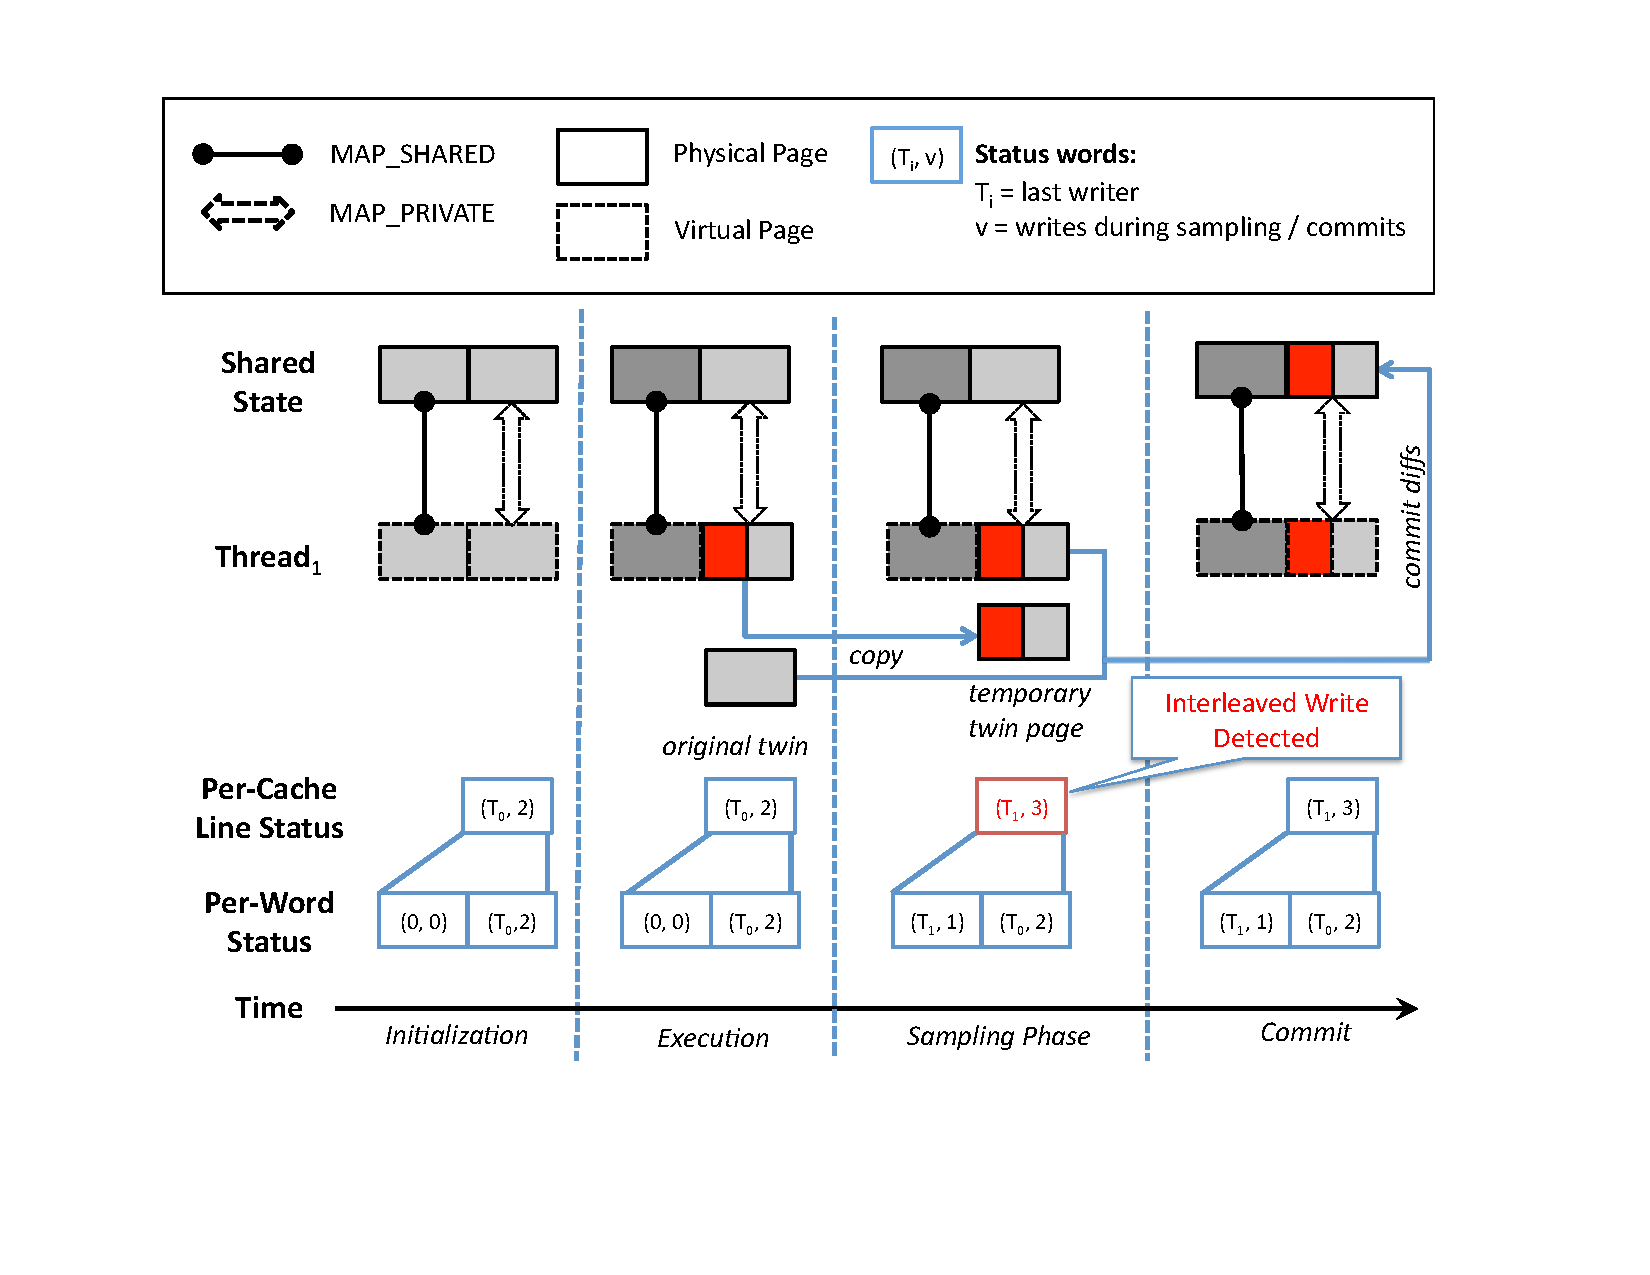
\includegraphics[width=6in]{sheriff/figure/sheriffdetective.pdf}
\caption{
Overview of \SheriffDetect{}’s operations. \SheriffDetect{} extends \Sheriff{} with sampling, per-cacheline status arrays, and per-word status arrays. For clarity of exposition, the diagram depicts just one cache line per page and two words per cache line.\label{fig:sheriffdetect}}
\end{figure*}

As discussed as in Section~\ref{sec:detectionidea}, we can detect cache invalidations only based on memory accesses: when we observe a memory access, we can update corresponding cache line status word, including recent memory access history and the number of cache invalidations on this cache line. When there is a memory access, we can check against its corresponding cache line status word to find out whether this memory access causes a cache invalidation or not. 

Since \SheriffDetect{} relies on the \sheriff{} framework to track memory writes. \sheriff{} framework provides a strong isolation of different threads' execution and only commits those changes of different threads to the shared mapping in the end of an transaction, by comparing a ``working'' page against its ``twin'' page as described in Section~\ref{sec:sherifftransaction}. Thus, \sheriffDetect{} can only detect write-write false sharing problems. 

Since the \sheriff{} framework only commits those local changes of different threads at synchronization points, it can only find those memory writes at synchronization points. 

However, if a transaction is long-running, finding memory changes at the end of a transaction is not enough to find those false sharing problems happening in the middle of a transaction. Actually, the \texttt{linear\_regression} benchmark (described in Section~\ref{sec:evaluation}), degrading the performance by more than $10\times$ because of its false sharing problem, only has a single transaction per thread. 

In order to detect memory writes in the middle of an transaction, \SheriffDetect{} employs a sampling mechanism, using the timer mechanism provided by the underlying operating system. We employs \texttt{alarm} mechanism to schedule an periodical alarm; whenever we get a \texttt{SIGALRM} signal, \SheriffDetect{} tracks memory writes in the current period using the twinning and diffing mechanism. To do this, \SheriffDetect{} also keeps and updates a ``temporary twin'' page to keep the content of a page at every alarm interval by simply copying from its ``working'' page, since a ``temporary twin'' page is always thread-private. The difference between a ``working'' page and its ``temporary'' page implies those memory writes happening in the current sampling period. 

Currently, \SheriffDetect{} samples memory accesses of each thread at every 10 microsecond, which is  adjustable in our implementation. More frequent sampling normally indicates more performance overhead. The tradeoff between the sampling period and performance overhead is further discussed and evaluated in Section~\ref{sec:results-sampling-overhead}. 

\subsubsection{Tracking Cache Invalidations}
\label{sec:invalidation}
As the discussion in Section~\ref{sec:detectionidea}, \SheriffDetect{} tracks and reports those cache lines with a big number of cache invalidations, where they are considered to cause serious performance problems. 

In order to track cache invalidations, \SheriffDetect{} introduces a cache line status word for every cache line of the globals and heap, showed in Figure~\ref{fig:cachelinestatusword}.  In this tool, every cache line status word contains two fields, the last thread writing to this cache line and the number of cache invalidations of this cache line. 
Every time, when \SheriffDetect{} detects a memory write, either at the end of transactions or in the sampling timer handler, it updates these two fields correspondingly. Based on the assumptions described in Section~\ref{sec:detectionidea}, \SheriffDetect{} increments the number of cache invalidations when there is a write from a different thread. To avoid using lock, \SheriffDetect{} updates those counters using atomic primitives. 

\subsection{Optimizations}

\SheriffDetect{} employs the following optimizations in order to reduce its performance overhead. 

\paragraph{Getting Callsite Information.}
\SheriffDetect{} intercepts memory allocation operations in order to collect callsites for every heap object. To reduce the performance overhead, \SheriffDetect{} do not use the bracktrace(), but identify the callsite by analyzing the return or frame address using GCC extensions. However, this can not work on applications without debugging information. 

\paragraph{Reducing timer overhead.}
As explained in Section~\ref{sec:memoryaccesses}, \SheriffDetect{} uses a sampling mechanism to track cache invalidations. To reduce the performance overhead caused by timer interruptions, \SheriffDetect{} activates sampling only when the average transaction time is larger than a threshold (currently 10 milliseconds). \SheriffDetect{} uses an exponential moving average to track the average transaction time ($\alpha = 0.9$). This optimization does not significantly reduce the possibility of finding false sharing since \SheriffDetect{}'s goal is to find an object with a large amount of interleaved writes from different threads.

\paragraph{Sampling to find shared pages.} 
To reduce the overhead, \SheriffDetect{} leverages a
simple insight: if two threads can falsely share a cache line, then they must simultaneously access the page containing this cache line. \SheriffDetect{} relies on page protection to determine whether pages are shared or not. If an application has a large number of transactions or a large memory footprint, the overhead of handling page protection can dominate the running time of running this application.

\SheriffDetect{} reduces its overhead by only tracking those shared pages, discovered by using another sampling mechanism. It is based on the following assumption: if objects on a page are frequently falsely shared, the corresponding page must also be frequently shared; thus, even with relatively infrequent sampling on memory accesses can detect those pages that are shared by multiple threads.  \SheriffDetect{} currently samples the first 50 out of every 1,000 periods (one period equals one transaction or one sampling interval). At the beginning of each sampling period, all memory pages are made read-only so that any
writes to each page will be detected. Upon finding a page that is shared across multiple threads, \SheriffDetect{} tracks all memory accesses happening on this page, thus possibly finding any false sharing inside this page. 

By using this sampling mechanism, those pages, with sharing status unknown, impose no protection overhead at all. \sheriffDetect{} only pays protection overhead for those shared pages outside the sampling period, instead of all memory pages. 

\subsection{Limitation}
\label{discussion:faultofdetect}

Unlike previous tools, \SheriffDetect{} reports no false positives, differentiates true sharing from false sharing, and avoids false positives caused by the reuse of heap objects. 

However, \SheriffDetect{} can under-report false sharing instances in the following situations:

\paragraph{Single writer.}
False sharing usually involves updates from multiple threads. But it can also arise when there is exactly one thread writing to part of a cache line while other threads read from it. Because \sheriffdetect{} can only track writes, it cannot detect the single-writer false sharing: one thread is writing to a cache line, while other threads are reading from this cache line. 

\paragraph{Heap-induced false sharing.}  
\sheriff{} replaces the standard memory allocator with one that, like the Hoard allocator, avoids most heap-induced false sharing. \sheriff{}'s memory allocator (like Hoard), carves memory into page-sized chunks; each thread allocates from its own set of chunks, and the allocator never splits cache lines across threads. Because \SheriffDetect{} uses a different custom memory allocator, it cannot detect false sharing that would be caused by using the standard memory allocator. Since it is straightforward to deploy Hoard or a similar allocator to avoid heap-induced false sharing, this limitation is not a problem in practice.

\paragraph{Misses due to sampling.}  Since it uses sampling to capture continuous writes from different threads, \SheriffDetect{} can miss writes that occur in the middle of sampling intervals. We hypothesize that false sharing instances that affect performance are unlikely to perform frequent writes exclusively during that time, and so are unlikely to be missed.
